\documentclass[letterpaper]{article}
\usepackage{fullpage} % smaller margins
\usepackage{graphicx}
\usepackage[utf8]{inputenc}
\usepackage{mathtools}
\usepackage{mathrsfs}
\usepackage{amssymb}
\usepackage{hyperref}
\usepackage[section]{placeins} % keep figures within their sections

\begin{document}
\title{Wavelet Transforms and Signal Processing}
\author{Jesse Connell}
\date{December 2014}
\maketitle

% \tableofcontents

\section{Overview}

An explanation of wavelets and their construction, use, and meaning can be challenging, simply because the field is so broad.
As Strang and Nguyen explain, perhaps a little blithely, ``a wavelet is a small wave'' \cite[p.~26]{strang}.
This simple phrase does capture the essential requirements for a wavelet:
a nonzero function with zero mean, and with localization in time and frequency. 
When used as vectors spanning a function space, wavelets allow functions to be projected onto them in order to learn from or work with the functions in more useful ways.
In particular, their localization in \emph{time}\emph separates wavelet methods from classic Fourier techniques.
Other than that, very few of the rules hold strict in all cases:
Characteristics like orthogonality and compact support may or may not be present,
and the dyadic tiling in the time/scale plane of the ``classic case'' is not necessarily the only structure possible.

In this limited space we will restrict ourselves to a subset of all these possibilities.
In particular we will focus on examples of 1D functions of time, like audio or bioelectric signals,
though the topic easily expands to signals in higher dimensions and other variables, like images across two spatial dimensions or video.
We focus on the simplest ``dyadic'' tiling in the time/frequency plane, corresponding to a logarithmic or ``octave'' decomposition \cite{strang}.
Numerical examples given here were created with MATLAB R2014b, using built-in tools and the Wavelet Toolbox.
(The encyclopedic depth of MATLAB's tools makes them invaluable for exploring the topic,
but open-source tools like Scientific and Numeric Python and community projects like PyWavelets \cite{pywavelets} are entering the space as well.
It will be interesting to see their progression in the near future.)

In terms of introductory texts, the breadth of interpretations and perspectives on the topic is striking.
In \emph{Wavelets and Filter Banks}, Strang and Nguyen present wavelets hand-in-hand with filter bank design, with matrix operations taking a lead role \cite{strang}.
They point out St\'{e}phane Mallat's discovery of this filter bank connection \cite[p.~33]{strang}, but
Mallat's own \emph{Wavelet Tour of Signal Processing} draws largely from a multiresolution perspective \cite{mallat}.
Goswami and Chan's \emph{Fundamentals of Wavelets} blend Hilbert space and multiresolution perspectives with matrix representations for discrete time cases \cite{goswami},
and Burrus, Gopinanth, and Guo's \emph{Introduction to Wavelets and Wavelet Transforms} alternates filter bank and Hilbert space viewpoints \cite{burrus}.
All of these perspectives yield insight on wavelets, and we will attempt to draw on some of that insight here.

Our goal here is to build up enough of the fundamental aspects of wavelets and wavelet transforms
so that the idea can be applied to an example case.
We first cover the basic motivation in going beyond Fourier analysis,
and explore the multiple viewpoints on the topic.
We include a brief comparison of some of the simplest wavelet systems to emphasize
the inherent trade off in time and frequency with any analysis method.
We end with a basic attempt at using the wavelet transform in a practical signal processing application: denoising an acquired biological signal.
We also touch on an example in the literature of applying wavelets for the compression, as opposed to denoising, of these signals.

\section{Fundamentals}

\subsection{Motivation}

Mallat refers to the ``indisputable hegemony of the Fourier transform'' with its reliance on a time-invariant operator,
despite our interest in the transient parts of a signal \cite[p.~1]{mallat}.
The ability to pick transients out of a time-varying signal has a multitude of examples, but to give one:
consider a signal with sharp peaks at specific times combined with constant tones across all times.
By eye or ear, we can see or hear the ``clicks'' in the signal and separate them from the constant tones.
The usefulness of wavelets can be phrased as the ability to match that intuition with mathematical rigor.

We are used to the idea of presenting a logarithmic frequency axis for Fourier transforms,
but the transform itself produces a linear range of evenly-spaced frequencies.
This does \emph{not} match our own intuition about what constitutes a logical spacing of frequencies!
An ``even spacing'' of frequencies when moving from one note to a higher octave and to the next higher octave is
a \emph{doubling} of frequencies with each increase.
As the equally-spaced lines on the staff of written music reveal,
what intuitively appears to be an equal frequency range compared to the one below is actually a range \emph{twice as large}.
This implies that our own ``frequency resolution'' decreases logarithmically as frequency increases.
In his article on Wavelets for American Scientist, Strang explains the doubling that occurs in each increase of scale
in a wavelet representation in terms of a set of instruments contributing to a symphony.

In her \emph{Ten Lectures on Wavelets}, Ingrid Daubechies provides a visual explanation of the challenges of achieving
good localization in both time and frequency \cite[Fig.~1.3]{daub}, which Goswami and Chan refer to for their own example \cite[Fig.~4.5]{goswami}.
Following suit, this concise example is worth repeating here. 

Figure \ref{fig:clicks} shows a time-varying signal composed of three tones and three impulses, given by
\[
f(t) = sin(2 \pi v_1 t) + sin(2 \pi v_2 t) + sin(2 \pi v_3 t) + \alpha(-2 \delta(0) + \delta(t_1) -\delta(t_2))
\]
Where \( \alpha = 3, v_1 = 500 \mathrm{Hz}, v2 = 1 \mathrm{kHz}, v3 = 2 \mathrm{kHz}, t_1 = -2 \mathrm{ms}, t_2 = 2 \mathrm{ms} \),
\(\delta(t)\) being the Dirac delta.  Following the original example, our function was sampled at 8 kHz
and \( \delta(t) \) was approximated with 
\[
\delta[n] = \left\{ 
  \begin{array}{l l}
    1 & \quad n=0 \\
    0 & \quad n=1
  \end{array} \right.
\]
(The frequencies and amplitudes are chosen so that f(t) has zero-mean and the sine wave frequencies are evenly spaced on a logarithmic scale.)

Figure \ref{fig:stft} shows a set of short-time Fourier transform plots of \(f\), using hamming windows with 50\% overlap.
In each plot the window width is halved.
For very long windows, frequency resolution is dominant, and the transform approaches a traditional FFT.
The impulses are nowhere to be seen.
Since time resolution is so poor,
they only appear in the form of an even contribution at all frequencies, as implied by their own Fourier transform.
As window length is cut in half at each step,
the pure sine waves become doubly smeared out in frequency (and the maximum value as shown in the color bar correspondingly drops by 50\%.)
But now the impulses become visible;
we can simultaneously see their even spread across frequencies on the vertical axis and their occurrence in time on the horizontal.
As we continue to improve our time resolution with smaller windows,
we improve our localization of the impulses, but at the expense of frequency resolution.
Finally the separation between the three constant tones is lost,
just as we have finally achieved good localization of the impulses in time.
In the analysis of a signal, why can't we separately consider both the tones we hear over longer times,
and the events we detect over shorter ones?
We can, and in essence that analysis \emph{is} the wavelet transform.
\begin{figure}[h]
  \caption{Signal composed of three constant tones and three clicks}
  \centering
    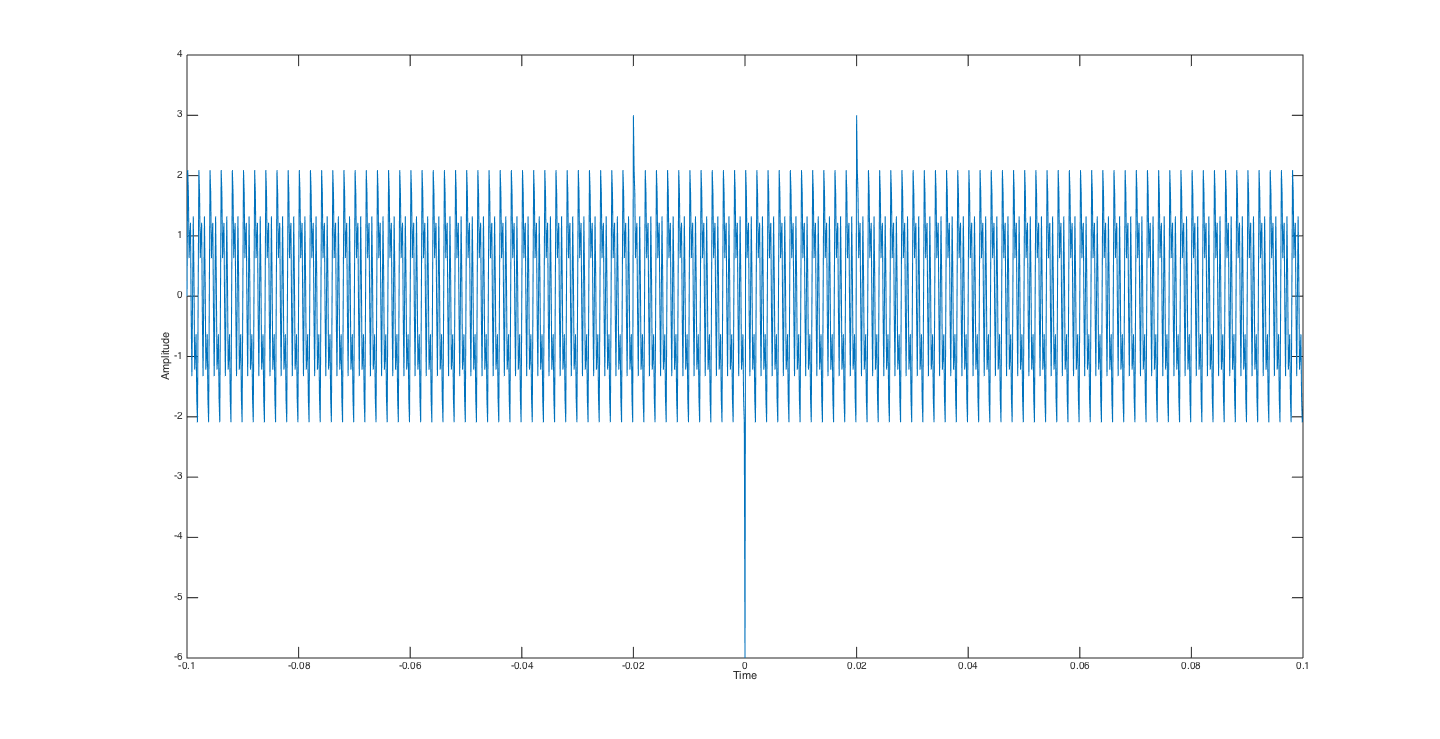
\includegraphics[width=0.8\textwidth]{figures/clicks}
  \label{fig:clicks}
\end{figure}
\begin{figure}[h]
  \caption{STFT with half-overlapping Hamming windows of varying widths}
  \centering
    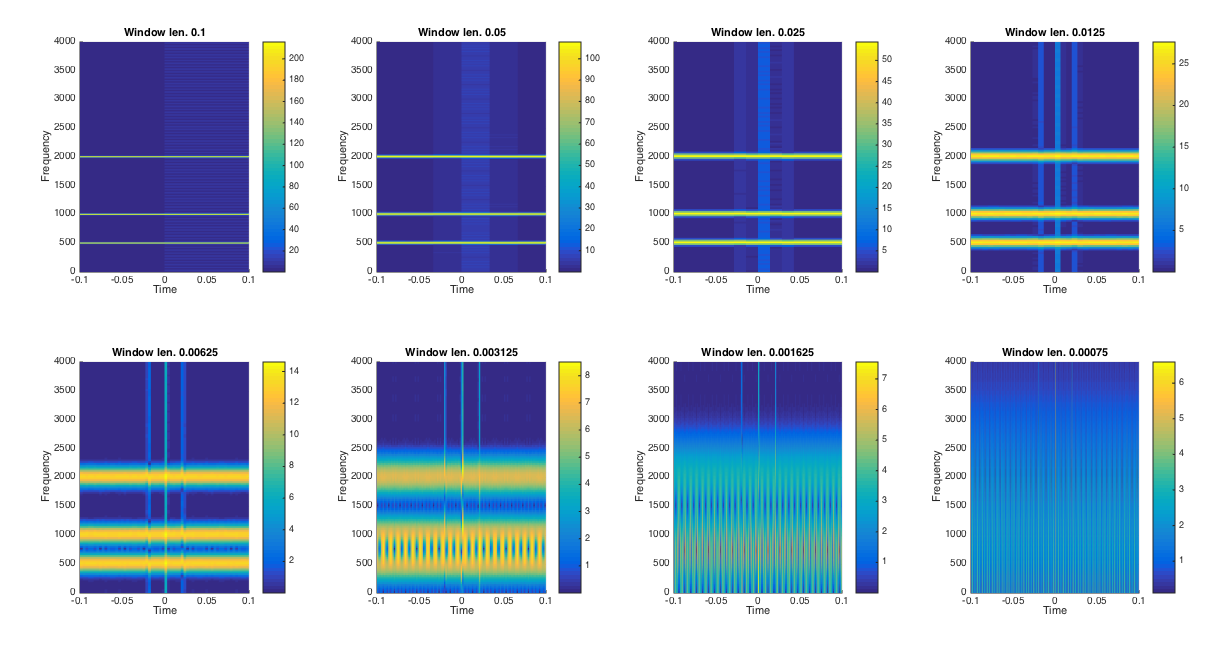
\includegraphics[width=1\textwidth]{figures/stft}
  \label{fig:stft}
\end{figure}
\begin{figure}[h]
  \caption{Magnitude of a continuous wavelet transform of \(f(t)\) with Morlet wavelet}
  \centering
    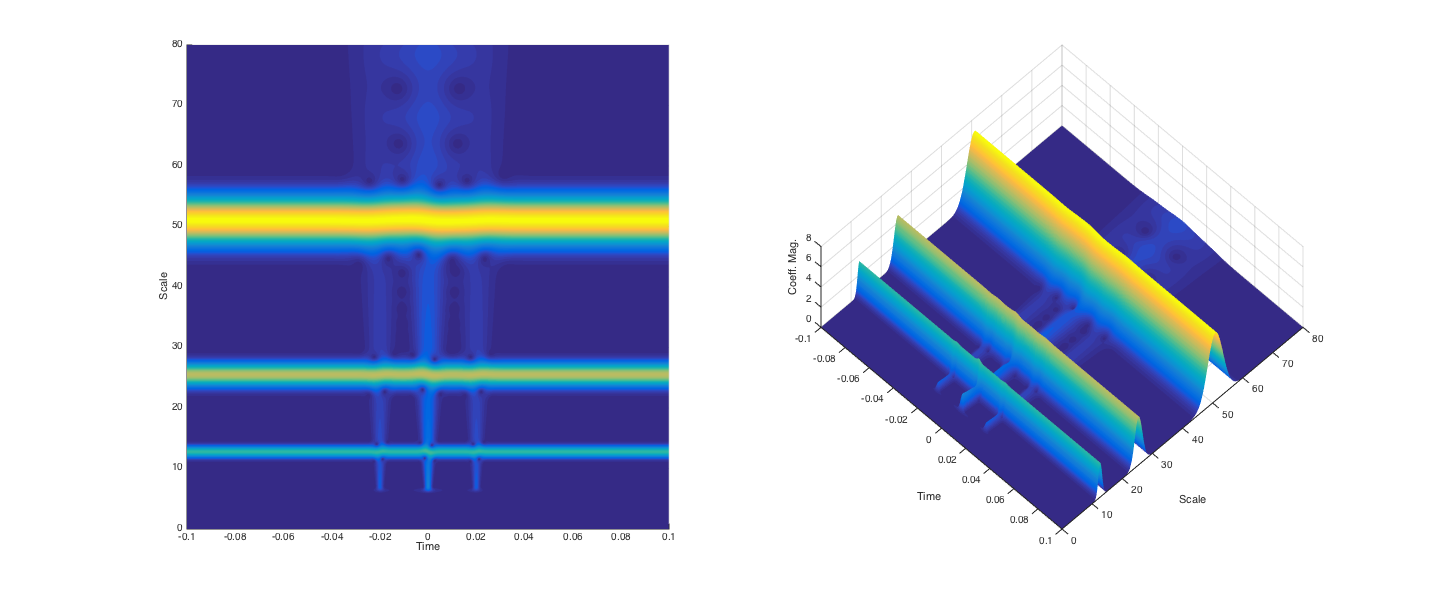
\includegraphics[width=1\textwidth]{figures/waveletclicks}
  \label{fig:waveletclicks}
\end{figure}

Figure \ref{fig:waveletclicks} shows the same signal considered earlier,
processed with a continuous wavelet transform, using a Morlet wavelet.
The idea of giving these different times and scales of detail their own time-varying functions,
and considering the subspaces these functions span relates to the multiresolution analysis perspective.
Our analysis at one level of detail can contribute to our analysis at the following level,
with this iterative process implemented in filter bank design.
Each of these views contributes to a cohesive and powerful method for signal processing. 


\subsection{Hilbert Space and Multiresolution Viewpoint}
Even if the practical aspects of implementing a wavelet system computationally occurs in discrete, finite dimensions,
an infinite-dimensional representation can provide key insights into the ideas.
Viewing a set of wavelet functions as vectors in a Hilbert space allows us to use the properties of orthogonality between vectors,
the norm of a vector, and a change of basis vectors, applying them to continuous signals in time or space.

In a classic Fourier transform, each component vector in the basis is a different complex exponential
with the relation between the components given by the frequency \( \omega \):
\( f(\omega) = e^{i \omega t} \).
Since the inner product of any one of these functions with any other is zero, they are orthogonal to one another:
\[ \langle f(\omega_1), f(\omega_2)\rangle = \int_{-\infty}^{\infty} f^*(\omega_1)\cdot f(\omega_2) \,\mathrm{d}t = 0 , \omega_1 \neq \omega_2 \]
The norm or ``length'' of a component is not unity:
\[ ||f|| = \sqrt{\langle f, f\rangle} = \sqrt{\int_{-\infty}^{\infty} e^{-j\omega t} e^{j\omega t} \,\mathrm{d}\omega } = \infty \]
But putting all these together, we do have a sort of orthonormality in this infinite-dimensional frequency domain:
\[ \langle f(\omega_1), f(\omega_2)\rangle = \int_{-\infty}^{\infty} f^*(\omega_1)\cdot f(\omega_2) \,\mathrm{d}t = \delta(\omega_1 - \omega_2) \]
By projecting a signal onto this new basis, we have effectively rotated it onto a new set of axes, but have kept the length of our ``vector'' the same \cite[p.~xi]{strang}.
As we can imagine geometrically in two dimensions (jumping ahead, Section \ref{sec:frames} draws on this for examples),
we can project onto a basis, scale the basis vectors using our projections, and sum the vectors for a round trip back to the original representation.

\subsection{Alfréd Haar's Creation}

In 1909 Alfr\'{e}d Haar published his PhD thesis, \emph{Zur Theorie der orthogonalen Funktionensysteme}.
Although terms like ``wavelets'' would make no appearance until decades later,
Haar's paper introduce what was later recognized to be a fundamental wavelet system.
In Chapter 3, Haar names ``the complete orthogonal function system \(\chi\), the most simple representative of
that class of orthogonal systems'' \cite{haar}.
Roughly seventy years later, Daubechies names entire families of wavelet functions of which Haar's wavelet 
can be seen as a starting point \cite[p.~16]{daub}.

In Haar's system, a particular family of piecewise linear functions can be used as a basis for
representing any given function of finite energy.
He used the pattern \(\chi_n^{(k)}(s)\) with $n$ and $k$ representing what are now referred to as scale and time.
\(\chi_0(s)\) is simply $1$ on the interval $[0,1]$, and \(\chi_1(s)\) is $1$ from $[0,\tfrac{1}{2})$
and $-1$ from $(\tfrac{1}{2},1]$.
In a more modern phrasing, \(\chi_0(s)\) is \(\phi(t)\), the scaling function,
and \(\chi_n^{(k)}(s)\) for $n>0$ is \(\psi_{j,k}(t)\), the wavelet function at each scale and time.
As scale increases by integers, the wavelet functions at that scale become shorter in time by a factor of $2$,
and amplitude higher by a factor of $\sqrt{2}$ (preserving norm).
The $k$ parameter delays these shortened functions in time.
Taken together, an expression relates the wavelet functions at higher scale to the lowest-scaled version, or
\emph{mother wavelet}:
\begin{equation}
\psi_{j,k}(t) = 2^{j/2}\psi(2^jt-k)
\end{equation}

Haar's insight was that, as this set of functions are orthogonal to one another and have unit norm,
we can project a function onto these scaled and shifted $\chi$ functions and obtain a complete description of the function in this new domain.
Here instead of $t$ (or $s$), we have $j,k$ (or $n,k$).
A synthesis expression for a time-domain function could be written as
\[
f(t) = \sum_{j,k} a_{j,k}\psi_{j,k}(t)
\]
And thanks to the orthonormality of the basis functions, we can determine the scaling coefficients $a_{j,k}$ with inner products,
or projections, onto those basis functions:
\[
a_{j,k} = \langle \psi_{j,k}(t), f(t) \rangle
\]
And finally, those Hilbert space projections have a simple integral form:
\[
\langle \psi_{j,k}, f(t) \rangle = \int_{-\infty}^\infty \psi_{j,k}^*(t)f(t)\,\mathrm{d}x
\]
(In this classic orthonormal wavelet basis, the same basic idea applies as in the Fourier example earlier,
but with a different change of variables instead of switching between pure time and pure frequency.)

Burrus, Gopinath, and Guo in particular use this to provide a foundation for the Hilbert space view of the transform \cite{burrus}.
(This is fitting, as Hilbert was Haar's thesis advisor \cite{hilbert}!)
Starting from Haar's simple scaling function, they introduce the vector spaces these scaled functions span.
A set of these time-shifted box functions at any given scale clearly also span the same spaces at each lower scale.
(Any function that could be built as the sum of a set of shifted boxes of one width could just as easily be built up using half-width boxes, for example.)
This means that the scaling functions are \emph{not} orthogonal, but rather, span nested spaces like Matryoshka dolls \cite[Fig.~2.1]{burrus};
a signal that falls entirely within the space spanned by scaling functions at one scale could also be projected solely onto the scaling functions at any higher scale.

Figure \ref{fig:ecgboth} shows an electrocardiogram recording (obtained from the ``PhysioBank ATM'' database of physiological signals \cite{physionet}).
The original signal over ten seconds is shown on the bottom plot.
The left four plots are projections onto the corresponding Haar scaling functions taken at higher and higher scales.
The scaling factors are multiplied by each version of the scaling function and superimposed, to give an approximation of the signal.
The right four plots show the signal projected onto the corresponding Haar wavelet functions at each of the same scales
(and superimposed on the corresponding vectors, as with the left plots).
On the left, increasing scale adds detail to the projection given at each lower scale, but also includes those same portions of the signal all over again.
These functions allow us to see increasingly fine detail, but don't perform any strict separation of the signal detail between scales. 
There is no method to make use of this as a signal processing technique with a ``round trip'' to an alternate basis and back to our original again.

Strang points out that in a discrete time-domain signal, we already have an implicit choice of basis \cite{strangwavelets};
this is simply the set of Dirac delta functions positioned at each possible time: \( \delta[t-t_0],\, t \in \mathbb{Z} \).
Any function in the time domain can be shown as a summation of scaled versions of each of these impulses.
What about an infinite-dimensional (continuous time) case?
Imagining taking scale to \( \infty \) in Burrus' example and the example plots here on the left side,
we know we should see our original signal represented again across time.
Taking the limit of the scaling function shows this as well:
% In Wolfram Alpha for k=0: http://goo.gl/jD8T32
\[ \lim_{j \to \infty} \phi_{j,k}(t) = \lim_{j \to \infty} 2^{j/2} (u(\tfrac{t}{2^j})-u(\tfrac{t-1}{2^j})) = \delta(t-k) \]
(where u(t) is the unit step function.)
Then projecting our signal onto this basis simply picks out every value across time, giving our original unique representation of the signal.
The scaling function sets the stage for a change of basis, but when looking across scales we haven't really ``gone'' anywhere yet.

If the space of signals that could be described by scaling functions at one level of scale is incrementally larger than that at the next lower scale,
we can gain more insight by looking at the \emph{differences} between one space and the next:
this is the space spanned by the corresponding wavelet functions at that scale!
In this way the the projections onto the wavelets at each scale tell us \emph{new} information,
entirely separate from the scales below,
because of the orthogonality of the wavelets between scales.
This is what the four right plots in Figure \ref{fig:ecgboth} show-- at each scale we have a new layer of information,
separate from what came before.

\begin{figure}[h]
  \caption{An ECG recording projected with increasing scale onto Haar's scaling functions on the left,
and Haar's wavelet functions on the right,
with original signal plotted at bottom.
(In practice the scaling function example was implemented by summing projections into the corresponding wavelet spaces up to each level;
The wavelet function example shows each individual level of scale separately.) }
  \centering
    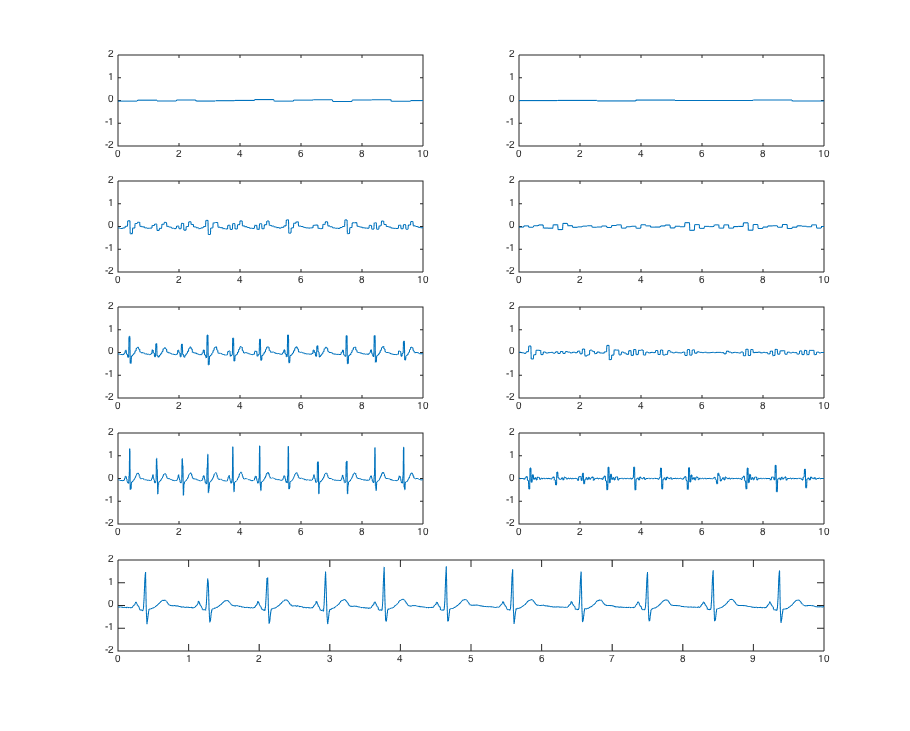
\includegraphics[width=1\textwidth]{figures/ecgboth}
  \label{fig:ecgboth}
\end{figure}

\subsection{Filter Bank Viewpoint}

In the practical case of finite, discrete time, matrix notation and the corresponding iterative filter banks
are both an effective explanation and a practical method of implementation.
At first we might simply see a finite list of values, for a vector in N-dimensional space: 
\(
\mathbf{x} = 
\begin{bmatrix}
x_1 & x_2 & x_3 & x_4
\end{bmatrix}^\mathrm{T}
\).
Our wavelet vectors, just like the functions before, are shifted and scaled versions of the mother wavelet:
\(
\psi_{J,K} = 2^{J/2}\psi[2^J n-K]
\) where \(\psi[n]\), the mother wavelet, is of the lowest-scale in the space.
Using the Haar wavelet, as before, this is
\( \psi[n] = \begin{bmatrix} 1/2 & 1/2 & -1/2 & -1/2 \end{bmatrix}^\mathrm{T} \).
Moving up to scale J = 1, we have two translations of a squeezed wavelet:
\( \psi_{1,0} = \begin{bmatrix} \tfrac{1}{\sqrt{2}} & -\tfrac{1}{\sqrt{2}} & 0 & 0 \end{bmatrix}^\mathrm{T} \)
and
\( \psi_{1,1} = \begin{bmatrix} 0 & 0 & \tfrac{1}{\sqrt{2}} & -\tfrac{1}{\sqrt{2}} \end{bmatrix}^\mathrm{T} \).
Clearly two increments of scale are all we can sensibly have in this limited space,
but the last missing piece is the scaling function itself at the ``very bottom'' in scale:
\( \phi = \begin{bmatrix} 1/2 & 1/2 & 1/2 & 1/2 \end{bmatrix}^\mathrm{T} \)

Following the geometric interpretation from before,
we \emph{could} project our signal vector onto each of these separately to get our coefficients.
For the scaling term, we have:
\[
\langle x[n],\phi[n] \rangle = \mathbf{x}\cdot\phi = 
\begin{bmatrix}
x_1 & x_2 & x_3 & x_4
\end{bmatrix}
\begin{bmatrix}
^1/_2 \\
^1/_2 \\
^1/_2 \\
^1/_2 \\
\end{bmatrix}
= ^1_2 x_1 + ^1_2 x_2 + ^1_2 x_3 + ^1_2 x_4
\]
And likewise for the wavelet projections:
% At J=0
\[
\langle x[n],\psi_{0}[n] \rangle = \mathbf{x}\cdot\psi_{0} = 
\begin{bmatrix}
x_1 & x_2 & x_3 & x_4
\end{bmatrix}
\begin{bmatrix}
^1/_2 \\
^1/_2 \\
-^1/_2 \\
-^1/_2 \\
\end{bmatrix}
= ^1_2 x_1 + ^1_2 x_2 - ^1_2 x_3 - ^1_2 x_4
\]
% At J=1, K=0
\[
\langle x[n],\psi_{1,0}[n] \rangle = \mathbf{x}\cdot\psi_{1,0} = 
\begin{bmatrix}
x_1 & x_2 & x_3 & x_4
\end{bmatrix}
\begin{bmatrix}
\tfrac{1}{\sqrt{2}} \\
-\tfrac{1}{\sqrt{2}} \\
0 \\
0 \\
\end{bmatrix}
= \tfrac{1}{\sqrt{2}} x_1 -\tfrac{1}{\sqrt{2}} x_2
\]
% At J=1, K=1
\[
\langle x[n],\psi_{1,1}[n] \rangle = \mathbf{x}\cdot\psi_{1,1} = 
\begin{bmatrix}
x_1 & x_2 & x_3 & x_4
\end{bmatrix}
\begin{bmatrix}
0 \\
0 \\
\tfrac{1}{\sqrt{2}} \\
-\tfrac{1}{\sqrt{2}} \\
\end{bmatrix}
= \tfrac{1}{\sqrt{2}} x_3 - \tfrac{1}{\sqrt{2}} x_4
\]

With these four dot products, we have the complete set of projections onto our alternate basis.
\emph{But this isn't the right way.}
We have repeated calculations across the projections.
A logical first step in seeing this more clearly is to structure the individual vectors of the basis into a matrix,
and the set of projections as the operation of this analysis matrix on our signal vector:
\[
\begin{bmatrix}
a \\
b \\
c \\
d \\
\end{bmatrix}
=
\begin{bmatrix}
^1_2                 &   ^1_2                 &   ^1_2                &  ^1_2                 \\
^1_2                 &   ^1_2                 &  -^1_2                &  -^1_2                \\
\tfrac{1}{\sqrt{2}}  &  -\tfrac{1}{\sqrt{2}}  &   0                   &  0                    \\
0                    &   0                    &  \tfrac{1}{\sqrt{2}}  & -\tfrac{1}{\sqrt{2}}  \\
\end{bmatrix}
\cdot
\begin{bmatrix}
x_1 \\
x_2 \\
x_3 \\
x_4 \\
\end{bmatrix}
\]
This isn't substantially different, but it lets us start to make observations about the transform as a whole.
Since each vector is orthogonal to each other vector and each has unit norm, the entire matrix is \emph{orthogonal},
and with that property we get other useful information: the inverse matrix is just the transpose.
If we start with our vector of coefficients and want to convert back into a time-domain signal, we simply use this inverse
synthesis matrix to reverse the transform.

If we break the previous matrix multiplication into two steps, we can avoid repeating the same calculations when finding the coefficients:
\[
\begin{bmatrix}
a \\
b \\
c \\
d \\
\end{bmatrix}
=
\begin{bmatrix}
^1_2                 &   ^1_2                 &   0                   &  0                    \\
^1_2                 &  -^1_2                 &   0                   &  0                    \\
0                    &   0                    &   1                   &  0                    \\
0                    &   0                    &   0                   &  1                    \\
\end{bmatrix}
\begin{bmatrix}
^1_2                 &   ^1_2                 &   0                   &  0                    \\
0                    &   0                    &   ^1_2                &  ^1_2                 \\
^1_2                 &  -^1_2                 &   0                   &  0                    \\
0                    &   0                    &  ^1_2                 & -^1_2                 \\
\end{bmatrix}
\cdot
\begin{bmatrix}
x_1 \\
x_2 \\
x_3 \\
x_4 \\
\end{bmatrix}
\]
Strang and Nguyen present this in a reduced notation \cite[p.~31]{strang}, emphasizing the sparsity of these individual matrices:
\[
\begin{bmatrix}
^1_2                 &   ^1_2                 &                       &                       \\
^1_2                 &  -^1_2                 &                       &                       \\
                     &                        &   1                   &                       \\
                     &                        &                       &  1                    \\
\end{bmatrix}
\begin{bmatrix}
^1_2                 &   ^1_2                 &                       &                       \\
                     &                        &   ^1_2                &  ^1_2                 \\
^1_2                 &  -^1_2                 &                       &                       \\
                     &                        &  ^1_2                 & -^1_2                 \\
\end{bmatrix}
\]
Using these sparse matrices allows the lower scale coefficients to be computed from the next higher scale, moving from maximum scale to zero.
The highest-scale wavelet coefficients are left as-is after the first iteration,
corresponding to the identity sub-matrix in the second iteration.
The only real computation in the second step is in using the previous scaling terms to find the ``lower detail'' wavelet and scaling coefficients at the next lower scale.
We can see the iteration even more clearly in an 8-dimensional case, while follow Strang and Nguyen's notation of \( r = \frac{1}{\sqrt{2}} \) (and noting that the higher exponents below yield \emph{smaller} components across each row, keeping each norm at unity) to give the full analysis matrix:
\[
\mathbf{A} = 
\begin{bmatrix}
r^3  & r^3  &  r^3  &  r^3  &  r^3  &  r^3  &  r^3  &  r^3  \\
r^3  & r^3  &  r^3  &  r^3  & -r^3  & -r^3  & -r^3  & -r^3  \\
r^2  & r^2  & -r^2  & -r^2  &  0    &  0    &  0    &  0    \\
0    & 0    &  0    &  0    &  r^2  &  r^2  & -r^2  & -r^2  \\
r    & -r   &  0    &  0    &  0    &  0    &  0    &  0    \\
0    & 0    &  r    & -r    &  0    &  0    &  0    &  0    \\
0    & 0    &  0    &  0    &  r    & -r    &  0    &  0    \\
0    & 0    &  0    &  0    &  0    &  0    &  r    & -r    \\
\end{bmatrix}
\]
And split into the iterative form:
\[
\mathbf{A} = 
\begin{bmatrix}
 r   &  r   &       &       &       &       &       &       \\
 r   & -r   &       &       &       &       &       &       \\
     &      &  1    &       &       &       &       &       \\
     &      &       &  1    &       &       &       &       \\
     &      &       &       &   1   &       &       &       \\
     &      &       &       &       &  1    &       &       \\
     &      &       &       &       &       &  1    &       \\
     &      &       &       &       &       &       &  1    \\
\end{bmatrix}
\begin{bmatrix}
 r   &  r   &       &       &       &       &       &       \\
     &      &  r    &   r   &       &       &       &       \\
 r   & -r   &       &       &       &       &       &       \\
     &      &  r    &  -r   &       &       &       &       \\
     &      &       &       &   1   &       &       &       \\
     &      &       &       &       &  1    &       &       \\
     &      &       &       &       &       &  1    &       \\
     &      &       &       &       &       &       &  1    \\
\end{bmatrix}
\begin{bmatrix}
 r   &  r   &       &       &       &       &       &       \\
     &      &  r    &   r   &       &       &       &       \\
     &      &       &       &   r   &   r   &       &       \\
     &      &       &       &       &       &  r    &  r    \\
 r   & -r   &       &       &       &       &       &       \\
     &      &  r    &  -r   &       &       &       &       \\
     &      &       &       &   r   &  -r   &       &       \\
     &      &       &       &       &       &  r    & -r    \\
\end{bmatrix}
\]
Using \( 8 = 2^3 \) dimensions shows the logarithmic nature of the process; for eight dimensions, we generalize the input signal three times,
scaling values down by a factor of \( \sqrt{2} \) to maintain unit norm for each more general projection than the one before.
Strang and Nguyen use this pattern to show two key points:
this iterative multiplication of sparse matrices \emph{is itself} the Fast Wavelet Transform, the wavelet equivalent of the Fast Fourier Transform;
and, iteratively applying these sums and differences against recursively generalized or ``abbreviated'' forms of our signal
is naturally the same as using an iterative filter bank with a logarithmic tree structure.

%In the filter bank view
With each piece of a filter bank we have an impulse response with its own coefficients.
Strang and Nguyen explain that the analysis matrix here corresponds to the iteration of averaging and differencing filters
with two coefficients, with the output of the averaging process passed on for more averages and differences.
The components are related to one another through the high/low frequency splitting (averaging and differencing) and downsampling,
but what other coefficients could we use, corresponding to what other filters and what other wavelets?
They move on to explain how more intricate filters can be matched with more advanced wavelet functions;
for now we stay with our simple case, but touch on its limitations below.

\subsection{Duality of Haar and Sinc Wavelets}

Switching our domain from pure time to pure frequency shows the limitation in applying Haar's system
as a signal processing technique.
To do this we take the Fourier transform of the most basic Haar wavelet,
and consider how the function changes in the frequency domain as we vary scale.
To start with, our mother Haar wavelet can be written as
\[
\psi(t) = [u(t) - 2u(t-\tfrac{1}{2}) + u(t+1)]
\]
Using the standard trick for time derivatives and Fourier transforms
(\( \frac{df}{dt} \) transforms to \( i\omega F(\omega) \) \cite[Eq.~2.21]{mallat}),
we can switch to a derivative form of the wavelet, take the transform, and switch back.
First, for the derivative and its transform:
\[
\frac{d\psi}{dt} = \delta(t) - 2\delta(t -\tfrac{1}{2}) + \delta(t - 1)
\]
\begin{align*}
\mathcal{F}(\frac{d\psi}{dt}) &= \int_{-\infty}^\infty \frac{d\psi}{dt} \, \mathrm{e}^{-i\omega t}\,\mathrm{d}t \\
    &= \int_{-\infty}^\infty 
  \left[\delta(t) - 2\delta(t -\tfrac{1}{2}) + \delta(t - 1)\right]\, \mathrm{e}^{-i\omega t}
\,\mathrm{d}t \\
    &=  \mathrm{e}^{-i \omega 0} -2 \mathrm{e}^{-i \omega \frac{1}{2}} + \mathrm{e}^{-i \omega 1} \\
    &=  1 - 2 \mathrm{e}^{-i \omega \frac{1}{2}} + \mathrm{e}^{-i \omega} 
\end{align*}
Then, for the transform of \(\psi\):
\begin{align*}
\Psi = \mathcal{F}(\psi) &= \frac{1}{i\omega} \mathcal{F}(\frac{d\psi}{dt}) \\
               &= \frac{1}{i\omega} -\frac{2}{i\omega} \mathrm{e}^{-i \omega \frac{1}{2}} + \frac{1}{i\omega} \mathrm{e}^{-i \omega}
\end{align*}
Finally, if we take into account time scaling \cite[Eq.~2.20]{mallat}, we have a general form for a Haar wavelet in the frequency domain:
\begin{align*}
\Psi(2^j t) &= \mathcal{F}(\psi(2^j t)) = 2^{-j} \Psi(2^j\omega) = 2^{-j} \left[
    \frac{1}{i 2^j \omega} -\frac{2}{i 2^j \omega} \mathrm{e}^{-i 2^j \omega \frac{1}{2}} + \frac{1}{i 2^j\omega} \mathrm{e}^{-i 2^j \omega}
\right] \\
   &= \frac{i 2^{-2j}}{\omega} \left[ 2\mathrm{e}^{-i2^j\omega\frac{1}{2}} - \mathrm{e}^{-i2^j\omega} - 1 \right]
\end{align*}
So, we have a function that drops off in magnitude with increasing frequency as \( |\tfrac{1}{\omega}| \) \cite[p.~10]{daub},
but higher scale stretches the frequency axis, effectively slowing the decay.
Figure \ref{fig:haartrans3} shows plots of the magnitude against frequency for increasing scale.
The large pair of peaks marks the Haar wavelet's localization in frequency,
but it starts poor and gets worse with the stretching of the axis.
\begin{figure}[h]
  \caption{Magnitude of Fourier transform of Haar wavelet}
  \centering
    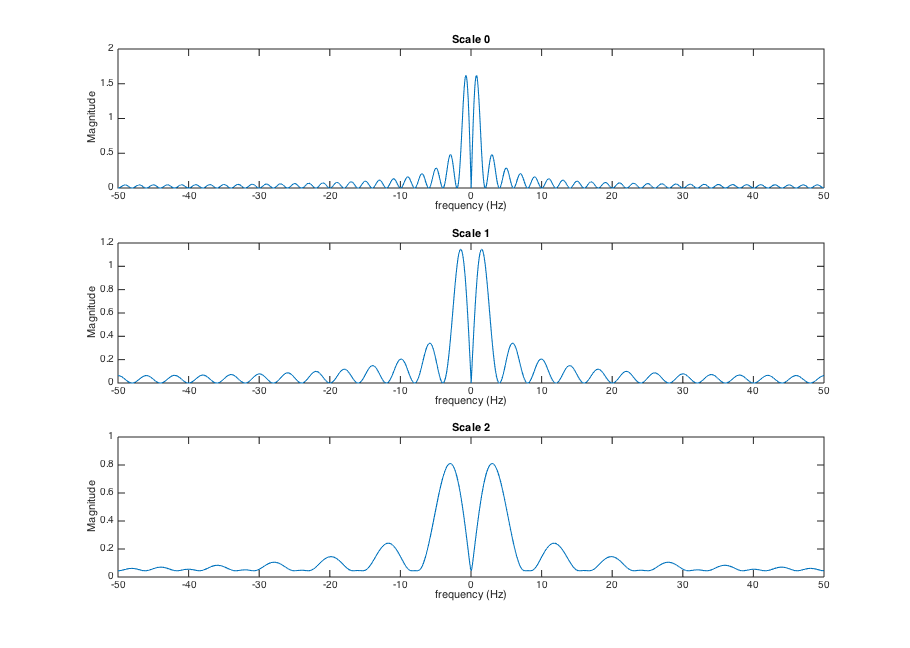
\includegraphics[width=1\textwidth]{figures/haartrans3}
  \label{fig:haartrans3}
\end{figure}
This is the downside of the trivially-simple compact support we have in the time domain for the Haar wavelets:
the sharp angles of these functions have considerable spread in frequency.
Wavelets provide more flexibility in working around the uncertainty principle,
but we can't escape it;
compact support in one domain precludes it in the other.

But, what if we start off with a simple, compactly-supported function in the frequency domain instead?
Strang and Nguyen pass through the topic only briefly, on the basis that actually implementing a filter with such a frequency response
would necessarily have infinite impulse response \cite[p.~51]{strang}, i.e., could \emph{not} be compactly supported in time.
But as a logical partner to Haar in the frequency domain, it is worth considering.
Figure \ref{fig:sinctrans3} shows the ideal case of a frequency-domain function that,
used as a filter on an input signal, would partition the signal into octaves with each increase in scale in the time domain.
Unlike in the Haar case, this corresponds to a perfect alignment between \emph{scale} and \emph{frequency}.

But now that we have this ``perfect alignment'' in frequency, we no longer have it in time:
as referred to earlier, the time-domain function for such a wavelet has infinite support.
Even though most of a projection's value is localized in time,
it still draws on the value of an input signal at \emph{all times}.
We have traded time-domain simplicity for frequency-domain simplicity,
gaining one by losing the other.
This emphasizes the limitations of taking a simplistic view of the ``time-frequency tiling'' idea.
(Mallat makes this idea concrete with a proof by contradiction, 
attempting to define an expression for a function with compact support in both domains
and obtaining a conflicting result for the time domain function
\cite[Theorem~2.6]{mallat}.)
One last observation here:
Considering when we would have a balance between time and frequency yields the \emph{Gabor wavelet},
with very similar expressions in both and frequency \cite[Eq.~4.62]{mallat}:
\[
g(t) = \frac{1}{(\sigma^2 \pi)^{1/4}} \mathrm{exp}\left(\frac{-t^2}{2 \sigma^2}\right)
\]
\[
G(\omega) = (4 \sigma^2 \pi)^{1/4} \mathrm{exp}\left(\frac{-\sigma^2\omega^2}{2}\right)
\]

\begin{figure}[h]
  \caption{Magnitude of Fourier transform of Sinc wavelet}
  \centering
    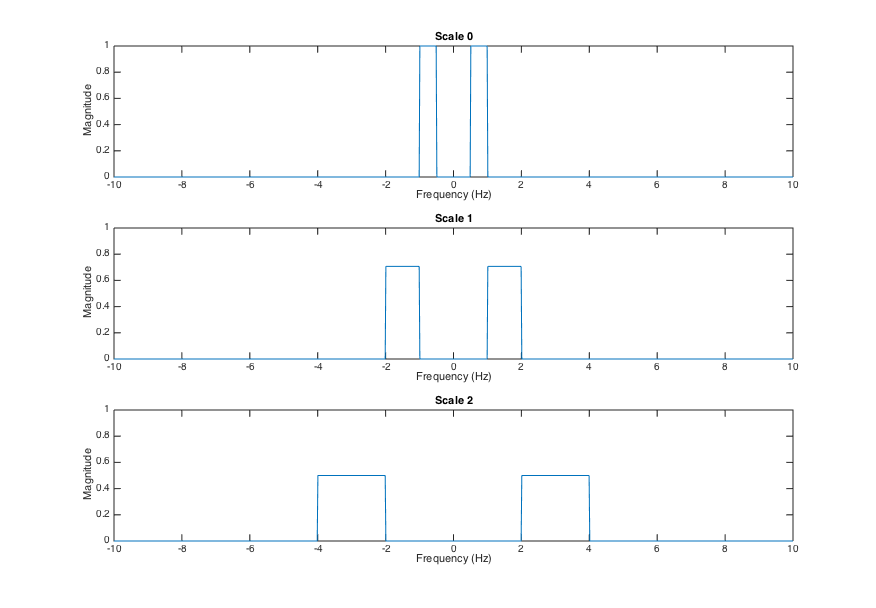
\includegraphics[width=1\textwidth]{figures/sinctrans3}
  \label{fig:sinctrans3}
\end{figure}

% What was this equation for??
%\begin{equation}
%a_{j,k} = \int_{k}^{k+\tfrac{1}{2}} f(t)\,\mathrm{d}t + \int_{k+\tfrac{1}{2}}^{k+1} f(t)\,\mathrm{d}t
% = F(t) \Big|_{k}^{k+\tfrac{1}{2}} - F(t) \Big|_{k+1/2}^{k+1}
% = 2F(k+\tfrac{1}{2}) - F(k) - F(k+1) \Big|_a^b
%%\langle \psi_{j,k}, f(t) \rangle = \int_{-\infty}^\infty \psi_{j,k}^*(t)f(t)\,\mathrm{d}x
%\end{equation}


\subsection{A Note about Frames}
\label{sec:frames}

Mallat introduces a frame as a family (more general than a ``basis'') of Hilbert space vectors that is \emph{not} orthonormal,
but which still maintain restrictions on the partitioning of a signal's energy when projected onto the vectors \cite[p.~126]{mallat}:
\[ A||f||^2 \leq \sum_{n \in \Gamma} |\langle f, \phi_n\rangle|^2  \leq B||f||^2 \]
In this case the norm of the vector in the new space isn't guaranteed, and we can only say that it falls within a \emph{range} between A and B.
If A and B are the same, the energy is always scaled by the same factor, and the frame is ``tight.''

A two-dimensional analog to this would be a set of more than two vectors that lie on different lines
(i.e, are not orthogonal but are not linearly dependent) as shown in Figure \ref{fig:frames2dproj}.
Projecting a vector in our 2D space onto these \emph{does} give a unique representation,
but we can't simply add the resulting projections together to get our original vector back.
One issue is that the resulting vector is scaled by some factor that falls between A and B.
% Mallat p 132
(Strang and Nguyen provide a clear explanation for how we can get back to our original vector:
we need a second family of vectors, \( \tilde{\phi}_{n} \), for which \( \langle \tilde{\phi}_{n,i}, \phi_{n,j} \rangle = \delta(i-j) \).)
The scaling factor given by the lower bound A is in a sense a measure of the redundancy of the frame in the space it spans \cite[p.~57]{daub}.
In two dimensional space, we can imagine projecting a vector onto three nonorthogonal unit vectors pointing in different directions,
and observe the "redundancy factor" by looking at both the original norm of the vector and the sum of the squares of the projections.
In Daubechies' two-dimensional example, we have three evenly-spaced vectors,
\( 120^{\circ} \) apart, which gives a tight frame with a redundancy of 3/2.
Figure \ref{fig:framesnorm} shows a few other examples in 2D on the left panels.
The right panels show the effect of projections onto these frames using a ``test vector''
of unit length with angle ranging from 0 to \(2\pi\).
The ``bad'' choice of uneven spacing between vectors in the frame (in the bottom pair of plots)
shows a varying effect on this test vector that depends on angle, corresponding to the A and B in the Hilbert space representations.

\begin{figure}[h!]
  \caption{Projection of an example vector (blue line) onto a frame (three red lines) in two dimensional space}
  \centering
    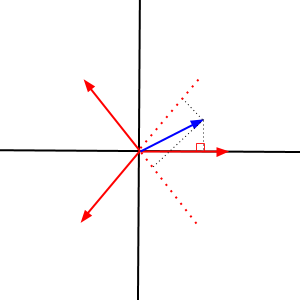
\includegraphics[width=0.25\textwidth]{figures/frames2dproj}
  \label{fig:frames2dproj}
\end{figure}

\begin{figure}[h]
  \caption{Effect of different frames on the norm of vectors rotated around the unit circle.
The first three frames have evenly-spaced vectors in angle,
while the last has an uneven distribution of three vectors around the unit circle (0, $\frac{5 \pi}{8}$, $\frac{11 \pi}{8}$).}
  \centering
    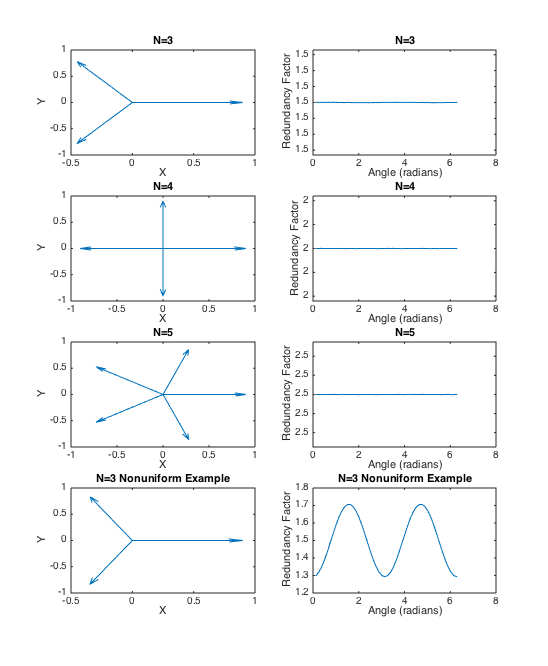
\includegraphics[width=0.7\textwidth]{figures/framesnorm}
  \label{fig:framesnorm}
\end{figure}

But what is the value in introducing this extra complication?
With \( A,B > 1 \), we have redundancy in our representation, since individual components could be substituted with scaled sums of one another. 
Intuitively this seems undesirable, since we have a clean, two-way transform with an orthonormal basis.
Mallat points out that redundancy can be beneficial if the \emph{projections onto the frame components themselves} are noisy in some way.
A thought of where we might see this issue arise is when implementing the transform numerically.
We must be concerned about the stability of the methods,
taking into account the effect of small perturbations \cite[p.~55]{daub}.
Without frames, performing and reversing the transform numerically could leave us far from where we started,
simply from round-off error.
\emph{Frames allow us to make the method numerically stable and robust} \cite[p.~56,~p.~98]{daub}.
% comparison with nyquist rate? Daub p53
% Strang p69, p208

\section{Applications}

\subsection{A Basic Attempt at ECG Denoising}

\begin{figure}[h]
  \caption{Example ECG waveform on top, with 60 Hz noise (in the form of a pure sine wave) added to the signal on the bottom.}
  \centering
    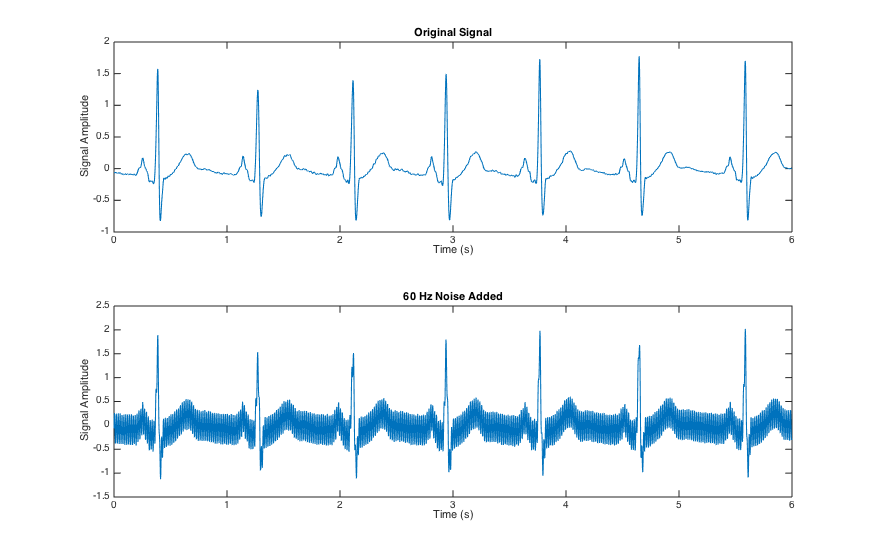
\includegraphics[width=1\textwidth]{figures/ecgplots}
  \label{fig:ecgplots}
\end{figure}

Figure \ref{fig:ecgplots} shows another view of the same electrocardiogram waveform shown on page~\pageref{fig:ecgboth}.
The upper plot shows six seconds of the original recording.
In the bottom plot, a 60 Hz sine wave has been added to the signal,
as a crude simulation of a recording with power line noise overlaid --
mimicking a commonplace filtering task in acquiring these sorts of signals.

In the simplest case, we could use a traditional lowpass filter 
(implemented in hardware with simple passive components, or software as a moving average)
and smooth out the added noise.
The cutoff frequency would be midway between the bulk of the signal content and noise.
A lower cutoff gives a smoother signal, but taken too far, the higher-frequency components of the signal are filtered too.
In practice the large sharp peak (the QRS complex) suffers most obviously, since its sudden change in time correspond to
energy at higher frequencies.
Figure \ref{fig:ecgmovavg} shows this problem visually:
as we increase window size from one plot to the next for a greater effect in a moving average filter,
the main peak in each cycle becomes increasingly filtered along with the noise.

\begin{figure}[h]
  \caption{A set of software-based moving averages on the noisy version of the signal.}
  \centering
    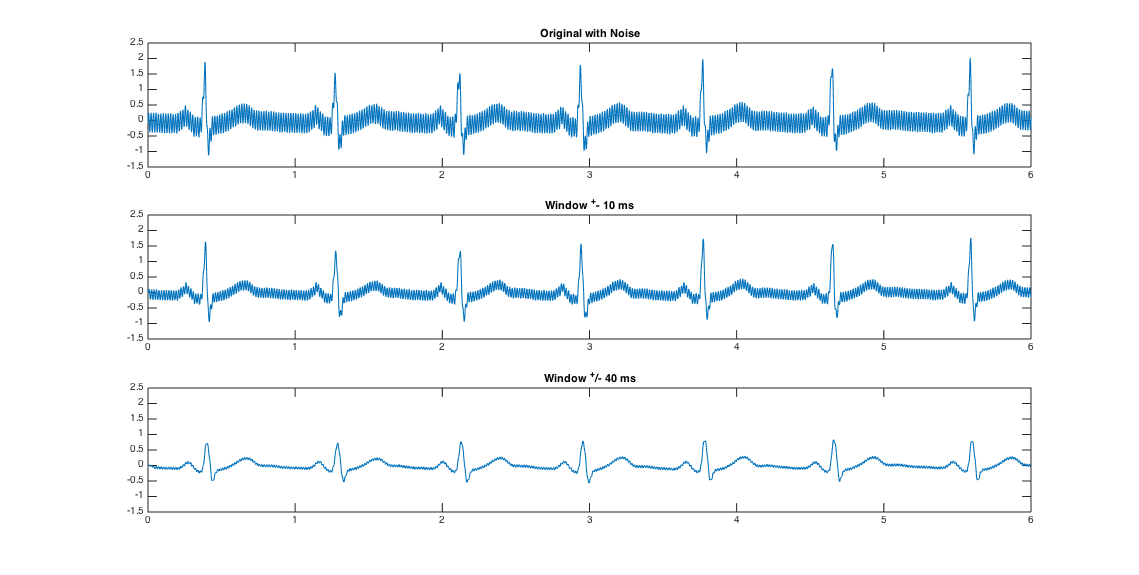
\includegraphics[width=1\textwidth]{figures/ecgmovavg}
  \label{fig:ecgmovavg}
\end{figure}

More complex linear filtering techniques can improve on this trade-off with more abrupt separation in the frequency domain,
but the change in amplitude at location of the QRS peaks raises an interesting point:
can we separate signal from noise by taking into account \emph{amplitude of frequency components at specific times},
when both our noise and components of our signal could be in similar frequency ranges?
Yes!  Burrus, Gopinath, and Guo describe exactly this strategy under the heading of
``Nonlinear Filtering or Denoising with the DWT'' \cite[Sec.~10.3]{burrus}.
A straightforward technique is \emph{hard thresholding} of coefficients in the wavelet domain;
as presented in \cite{burrus}, for wavelet coefficients $Y$, this is:
\[
\hat{X} = T_h(Y,t) = \left\{ 
  \begin{array}{l l}
    Y, & \quad |Y| \ge t \\
    0, & \quad |Y| < t
  \end{array} \right.
\]
Where taking the inverse transform to produce $x(t)$ creates the denoised time domain signal.
To implement a hard thresholding scheme for this simple trial,
we took a signal sampled at 500 Hz and truncated it as far as possible while still giving 
an even power-of-two split for $2^{14}$ samples (about 30 seconds).
A Haar wavelet decomposition using MATLAB's \texttt{wavedec} function was then taken up to scale 14  for ``full coverage''
(as scale 14 yields pointwise differences on the original signal).
A threshold was applied to the top three scales: coefficients above the threshold were left as-is
and coefficients below were removed.
The actual threshold value was taken fairly arbitrarily for this example to be 0.7, or about half of peak amplitude.
The altered coefficients were fed back into MATLAB's \texttt{waverec} function to synthesize the denoised signal back in the time domain.

Figure \ref{fig:ecgcleaned} shows the final result:
in this admittedly simplistic example, we did reach our goal!
The noise is removed, with minimal effect on the original signal.
(An occasional jagged edge in one QRS peak or another reveals that this is \emph{not} an LTI operation,
in terms of how frequency components are treated;
the thresholding implicitly makes high frequencies that occur at the times of the large peaks
different from those between peaks.)
The complexity of implementing the forward and reverse transforms comes with a clear benefit inside the new domain:
a concise expression for the change we want to apply that matches well with intuition.

\begin{figure}[h]
  \caption{The final result of attempted denoising of ECG signal with hard threshold in wavelet domain.}
  \centering
    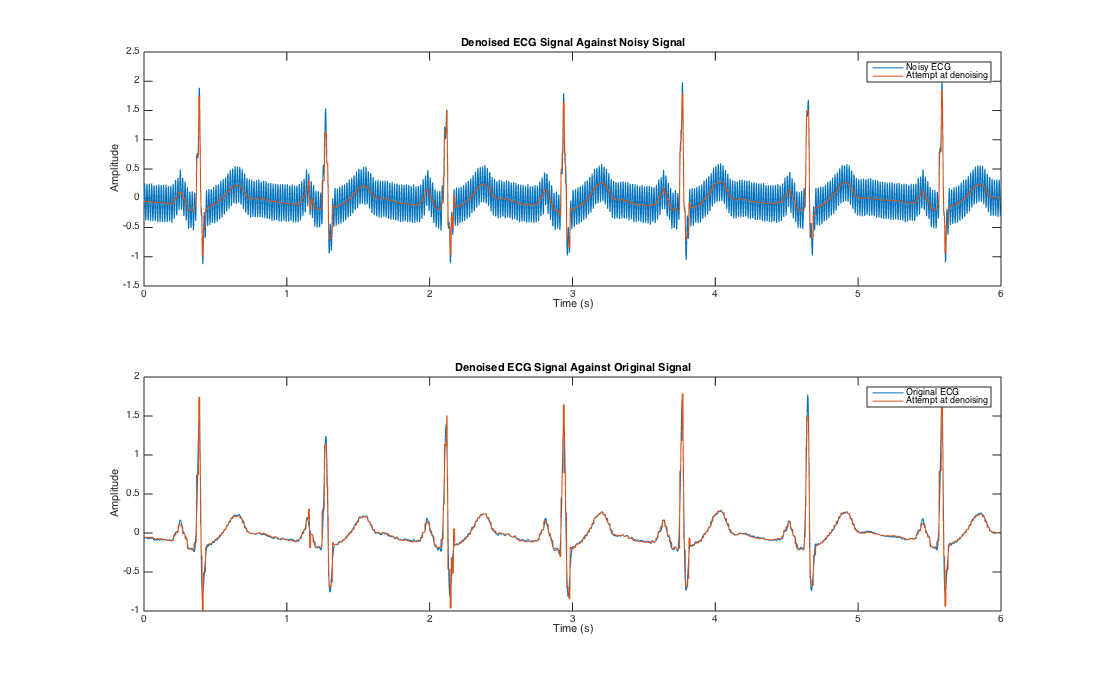
\includegraphics[width=1\textwidth]{figures/ecgcleaned}
  \label{fig:ecgcleaned}
\end{figure}

\subsection{ECG Compression}
Strang and Nguyen provide a brief application example in the form of \emph{compressing} electrocardiogram recordings \cite[p.~385]{strang},
drawing from Nguyen's research into the topic \cite{nguyenecg}.
To allow evaluation of the quality of the compressed signal, they use the percent RMS difference between original and compressed signals:

\[
PRD = \sqrt{\tfrac{\sum{x_{or}(n)-x_{re}(n)}^2}{\sum{x_{or}(n)}^2}}  \times 100\%
\]

(They point out that preservation of diagnostic details in the signal is the mark of successful compression, rather than low PRD per-se.
But, the PRD does allow a point of objective comparison between different algorithms.)

Showing a comparison of compression techniques with varying effective bit rates, 
their compression technique shows an order of magnitude improvement in PRD compared to AZTEC,
another commonly-used ECG compression system.
This is easily confirmed in the example plots showing the same 2.5 second recording compressed with several methods;
both non-wavelet methods suffer from distortion in the form of sudden jumps and blockiness in the signals.
The main strength in the application of the wavelet method is the flexibility of the basis function length;
varying length along with scale allows for a concise representation without the characteristic ``blocking'' of other methods \cite[p.~368]{strang}.
Referring back to an earlier example we see the same concept where other methods produce blocking or ringing in compressed images
due to discontinuities in the basis functions.

As with their example using images, the core of the compression technique for ECG signals is in
allocating bits in accordance with the relative partitioning of signal energy into the different components;
in the image case, Strang and Nguyen argue that, ``clearly, subimages with lower energy levels should have fewer bits.''
Rather than simply zeroing out coefficients that are considered negligible,
this shows a more nuanced approach,
where the resolution of the coefficients themselves is varied depending on their significance.
(This has a comparison with how a data acquisition system should provide dynamic range;
a given number of bits should be matched to signal amplitude to maximize resolution.)
Coefficients that are of the lowest significance can be allocated zero bits for their storage,
while coefficients that are larger can be stored with increasing quality.
The actual algorithm for assigning bits might consider any number of criteria (the authors mention distortion, energy, and entropy),
but the fundamental idea is the same.
The final step in the overall compression method is to group zero coefficients together
so that an entropy coding method can work effectively.
But, in terms of the wavelet-based approach, the central idea is in the quantization of the coefficients.
% page 368

\section{Concluding Remarks and Further Steps}

Reaching back to Haar's work around 1910, and culminating in a flurry of activity in the 1980's and 1990's,
wavelet techniques have matured into a recognized area of applied mathematics and signal processing.
In more recent years we can see this in the extensive support for wavelets in both commercial software,
as with MATLAB's Wavelet Toolbox \cite{wavelettoolbox}, and open-source and community implementations,
such as PyWavelets \cite{pywavelets}.
PyWavelets' author has also created a web-based ``dictionary'' of common wavelet families \cite{waveletbrowser}.

The range covered here has admittedly been limited.
We've focused on exploring the absolutely simplest structures that could be called wavelets,
trying to develop intuition into the main ideas and the most basic applications.
In practical usage so much more has been developing since Haar's work a century ago:
Ingrid Daubechies' work on more advanced compactly-supported wavelets,
the recognition of the connection to filter bank design by St\'{e}phane Mallat,
and additional wavelet structures like those proposed by Yves Meyer, to name a few.
As explored here very briefly, wavelet-based signal processing has particular strengths in
biomedical signal processing \cite[p.~218]{burrus};
an obvious next step is to investigate the usage of the more advanced and modern techniques
in this particular area.

\newpage
\bibliographystyle{alpha}
\bibliography{waveletrefs}

\end{document}
